% ---------------------------------------------------
% Trabajo Final de Grado
% Author: Eric Ríos Hamilton <alu0101549835@ull.edu.es>
% Chapter: Evaluation
% ----------------------------------------------------
\chapter{Evaluation} \label{chap:Evaluation}

The main form of evaluation chosen for this project will be execution time. 
As already explained in Section \ref{sec:quality_evaluation}, the development of a framework capable of evaluating the quality of the generated terrain lies outside of the realistic goals of this project.
However, an evaluation of the computational cost of each step and concrete algorithm in the generation process, as well as profiling during game execution, are well within it and appropriate. 

To achieve this, a benchmarking system has been developed.
Each benchmarking run is defined by a \href{{https://github.com/fsande/TFG---Eric-Rios/blob/main/Godot-TerrainGeneration/benchmarking/config/benchmark_profile.gd}}{\texttt{BenchmarkProfile}}\footnote{\href{{https://github.com/fsande/TFG---Eric-Rios/blob/main/Godot-TerrainGeneration/benchmarking/config/benchmark_profile.gd}}{\textit{Godot-TerrainGeneration/benchmarking/config/benchmark\_profile.gd}}}, which takes an array of \href{{https://github.com/fsande/TFG---Eric-Rios/blob/main/Godot-TerrainGeneration/terrain_generation/configuration/terrain_configuration.gd}}{\texttt{TerrainConfiguration}s}\footnote{\href{{https://github.com/fsande/TFG---Eric-Rios/blob/main/Godot-TerrainGeneration/terrain_generation/configuration/terrain_configuration.gd}}{\textit{Godot-TerrainGeneration/terrain\_generation/configuration/terrain\_configuration.gd}}}. 
The profiles are further customizable with parameters such as number of iterations, chunks to generate or warmup iterations.
The profile is then run by the \href{https://github.com/fsande/TFG---Eric-Rios/blob/main/Godot-TerrainGeneration/benchmarking/core/terrain_benchmark.gd}{\texttt{TerrainBenchmark}}\footnote{\url{https://github.com/fsande/TFG---Eric-Rios/blob/main/Godot-TerrainGeneration/benchmarking/core/terrain_benchmark.gd}} class, which repeatedly executes the different stages of generation for the selected configuration and records the execution time of each step, together with memory-related metrics associated primarily with cache usage.
The data is then processed into a \href{{https://github.com/fsande/TFG---Eric-Rios/blob/main/Godot-TerrainGeneration/benchmarking/core/benchmark_result.gd}}{\texttt{BenchmarkResult}}\footnote{\href{{https://github.com/fsande/TFG---Eric-Rios/blob/main/Godot-TerrainGeneration/benchmarking/core/benchmark_result.gd}}{\textit{Godot-TerrainGeneration/benchmarking/core/benchmark\_result.gd}}}, which can be stored as a CSV or JSON file.
Statistically meaningful values such as mean, standard deviation and interquartile ranges are calculated and recorded as well.
A Python program using Plotly\footnote{\href{https://plotly.com/python/}{Plotly Documentation} - \url{https://plotly.com/python/}} has also been developed to visualize the information in an interactive HTML file.

This Chapter can not, due to the limited extension of this work, include all the findings achieved thanks to the benchmarking system.
As such it will include only some of the most interesting observations made.
Further benchmarking information and generated reports are stored in the GitHub repository for the TFG \cite{URL::TFG} under the \textit{DataAnalysis} directory\footnote{\href{https://github.com/fsande/TFG---Eric-Rios/tree/25d1ed8639140cf9c2933ac497b0037b8fef1072/DataAnalysis}{\textit{DataAnalysis}} - \url{https://tinyurl.com/DataAnalysisDir}}.

Benchmarks, unless stated otherwise, have been performed on a Windows Desktop computer, with an {Intel(R) Core(TM) i7-14700KF CPU and a NVIDIA GeForce RTX 4060 Ti GPU.

\section{Heightmap Generation - CPU vs GPU}

The benchmarking results featured in Table \ref{tab:gpu_cpu_comparison} and visualized by Figure \ref{fig:heightmap_gen_cpu_gpu} clearly demonstrate the advantages of GPU-accelerated heightmap generation for large terrains. 
For a 5000 x 5000 pixels heightmap, the GPU implementation achieved a mean total pipeline execution time of 2471.24 ms, whereas the CPU implementation required 37653.96 ms, making the GPU version approximately 15.2x faster overall. 
The most significant difference can be observed in highly parallel image-processing operations such as the blur pass, where GPU execution averaged only 95.92 ms compared to 30331.9 ms on the CPU. 
Other operations, like combiners and contrast adjustment, also benefited substantially from GPU execution.
Operations such as those performed by \href{{Godot-TerrainGeneration/terrain_generation/heightmap/sources/image_heightmap_source.gd}}{\texttt{ImageHeightmapSource}}\footnote{\href{{Godot-TerrainGeneration/terrain_generation/heightmap/sources/image_heightmap_source.gd}}{\textit{Godot-TerrainGeneration/terrain\_generation/heightmap/sources/image\_heightmap\_source.gd}}}  or \href{{https://github.com/fsande/TFG---Eric-Rios/blob/main/Godot-TerrainGeneration/terrain_generation/heightmap/sources/noise_heightmap_source.gd}}{\texttt{NoiseHeightmapSource}}\footnote{\href{{https://github.com/fsande/TFG---Eric-Rios/blob/main/Godot-TerrainGeneration/terrain_generation/heightmap/sources/noise_heightmap_source.gd}}{\textit{Godot-TerrainGeneration/terrain\_generation/heightmap/sources/noise\_heightmap\_source.gd}}} are purely CPU driven, so the differences between runs visualized on the table are within expected measurement variance.
These results, as expected, strongly support the use of GPU compute pipelines for PCG workloads dominated by image-processing operations.

\begin{table}[H]
\centering
\begin{tabular}{lccc}
\toprule
\small\textbf{Stage} & \small\textbf{GPU Mean (ms)} & \small\textbf{CPU Mean (ms)} & \small\textbf{Speed-up} \\
\midrule
Total & 2494.20 & 37583.65 & 15.07x \\
Noise Source [type=5] & 1085.34 & 1106.58 & 1.02x \\
ContrastProcessor & 764.68 & 1936.32 & 2.53x \\
Blur (radius: 3.0) & 95.92 & 30331.90 & 316.22x \\
Noise Source [type=2] & 126.72 & 126.78 & 1.00x \\
Combiner Multiplication & 180.98 & 2211.46 & 12.22x \\
Image Source & 10.36 & 10.20 & 0.98x \\
Combiner Average & 208.66 & 1838.88 & 8.81x \\
Pipeline overhead & 21.54 & 21.53 & 1.00x \\
\bottomrule
\end{tabular}
\caption{Comparison of GPU and CPU execution times for heightmap generation (5000 x 5000 pixels) 50 samples each.}
\label{tab:gpu_cpu_comparison}
\end{table}


%% ===================================================
\begin{figure}[H]
    \centering
    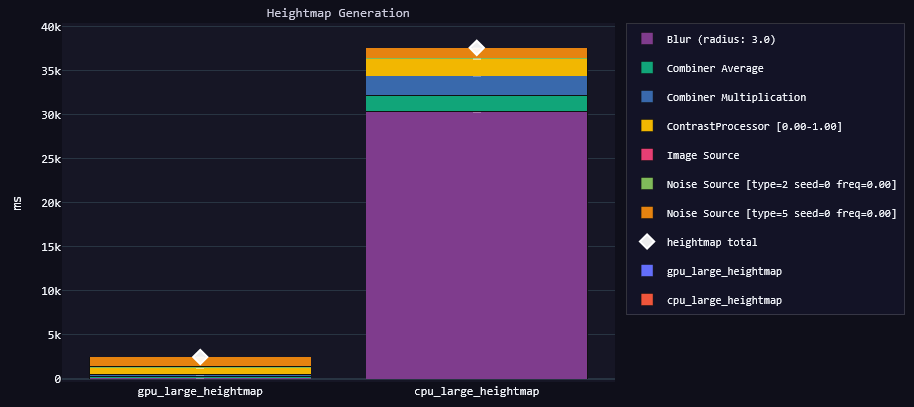
\includegraphics[width=1.0\textwidth]{Memoria/images/gpu_vs_cpu_large_heightmap.png}
    \caption{Comparison of GPU and CPU heightmap generation of 5000 by 5000 pixels.}
    \label{fig:heightmap_gen_cpu_gpu}
\end{figure}
%% ===================================================


\section{Chunk Generation - GDScript vs C++}
The implementation of chunk generation in C++ has shown significant benefits over the original GDScript one.
As evidenced in Figure \ref{fig:chunk_gen_gd_vs_cpp} the C++ implementation is noticeably faster.
The generation of a LOD 0 chunk with 256 subdivisions takes a mean execution time of 408.434 ms with the GDScript implementation and only 11.776 ms in C++.

%% ===================================================
\begin{figure}[H]
    \centering
    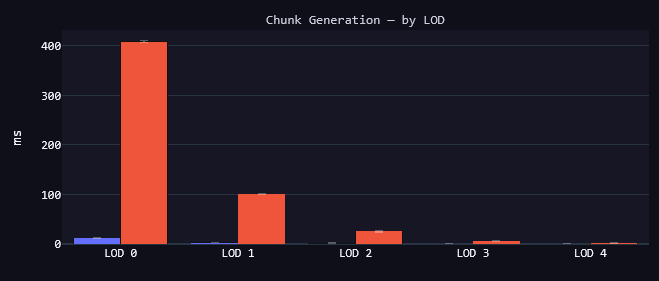
\includegraphics[width=1.0\textwidth]{Memoria/images/chunk_gen_gdscript_vs_cpp.png}
    \caption{Comparison of C++ (left, blue) and GDScript (right, orange) chunk generation time by LOD.}
    \label{fig:chunk_gen_gd_vs_cpp}
\end{figure}
%% ===================================================

As previously discussed, one of the primary motivations for migrating chunk mesh generation to C++ was to better exploit asynchronous execution, since the overhead and synchronization costs of GDScript limited the effectiveness of multithreading.
The data featured in Figure \ref{fig:async_chunk_gen} firmly supports the decision.

The GDScript implementation achieved noticeable gains under moderate concurrency, improving from 12.2 seconds sequentially to 7.06 seconds with four worker threads, amounting to a 1.73x speed-up.
However, despite the improvement, throughput remained low, at 4.25 chunks per second.
Increasing concurrency further up to 28 threads caused performance to collapse entirely.
Execution time increased to 21.4 seconds, making the asynchronous version approximately 1.76x slower than the sequential pipeline.
This points to synchronization overhead, runtime contention and thread management dominating execution at high concurrency.

In contrast to this, the C++ implementation demonstrated healthier scaling behaviour.
Sequential generation of 30 chunks completed in 346.5 ms, while four worker threads reduced execution time to 254.2 ms, a 1.36x speed-up over the sequential configuration.
Notably, a further increase of worker threads up to 28 did not improve performance, showing only a 1.34x speed-up over the sequential path.
This indicates that once chunk generation becomes sufficiently fast, parallelism's overhead begins to outweigh the benefits.

%% ===================================================
\begin{figure}[H]
    \centering
    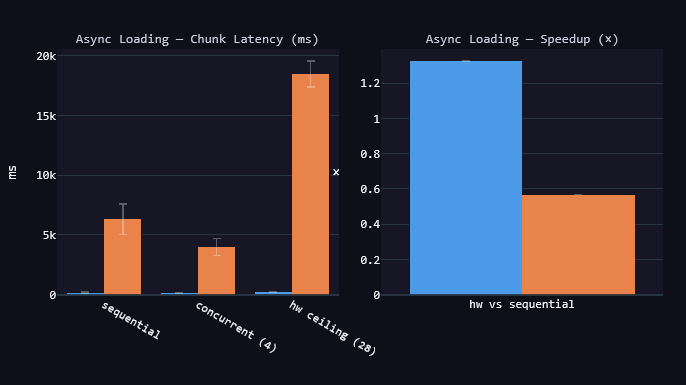
\includegraphics[width=1\textwidth]{Memoria/images/async_chunk_gen_cpp_vs_gd.png}
    \caption{Comparison of C++ and GDScript asynchronous chunk generation time.}
    \label{fig:async_chunk_gen}
\end{figure}
%% ===================================================

\section{Chunk Generation - GPU vs CPU}

The benchmarking results presented in Table \ref{tab:gpu_cpu_chunk_comparison} and partially visualized in Figure \ref{fig:gpu_vs_cpu_2000} reveal a more nuanced picture than the heightmap generation.
While the highly parallel image-processing operations present in heightmap generation greatly benefit from GPU computations, chunk mesh generation involves more sequential, geometry-focused work, which reduces the rate at which the GPU provides gains.

For a chunk of resolution 256, the CPU implementation achieved a mean generation time of 15.20 ms, while the GPU implementation required 20.29 ms, making the CPU nearly 1.33x faster.
This persists as LOD gets less detailed, with GPU dispatch and synchronization overhead dominating generation time at low resolutions and CPU being faster.

The situation changes at higher resolutions, such as 2000, where the GPU parallelization achieves a mean of 745.87 ms compared to the CPU's 819.63 ms, a modest 1.10x improvement.
As the detail decreases, however, the benefits disappear once again.

These results indicate that GPU acceleration only provides meaningful benefits 
for mesh densities large enough to amortize dispatch overhead. In practice, 
chunks are generated at far lower vertex densities than resolution 2000, meaning the 
CPU path will be faster for the vast majority of generation work, without even 
accounting for the threading benefits described in Section \ref{sec:chunking_and_lod}.

\begin{table}[H]
\centering
\begin{tabular}{cccccc}
\toprule
\small\textbf{Base} & \small\textbf{LOD} & \small\textbf{Effective} & \small\textbf{GPU Mean (ms)} & \small\textbf{CPU Mean (ms)} & \small\textbf{Speed-up} \\
\midrule
\multirow{5}{*}{256}  & 0 & 256 & 20.29 & 15.20 & 0.75x \\
                      & 1 & 128 &  8.95 &  3.80 & 0.42x \\
                      & 2 &  64 &  5.37 &  0.79 & 0.15x \\
                      & 3 &  32 &  5.47 &  0.21 & 0.04x \\
                      & 4 &  16 &  5.85 &  0.08 & 0.01x \\
\midrule
\multirow{5}{*}{2000} & 0 & 2000 & 745.87 & 819.63 & 1.10x \\
                      & 1 & 1000 & 199.16 & 214.04 & 1.07x \\
                      & 2 &  500 &  53.46 &  50.46 & 0.94x \\
                      & 3 &  250 &  16.58 &  12.59 & 0.76x \\
                      & 4 &  125 &   6.73 &   2.55 & 0.38x \\
\bottomrule
\end{tabular}
\caption{Comparison of GPU and CPU chunk generation times and speed-up by resolution and LOD level (25 samples each).}
\label{tab:gpu_cpu_chunk_comparison}
\end{table}

%% ===================================================
%\begin{figure}[H]
%    \centering
%    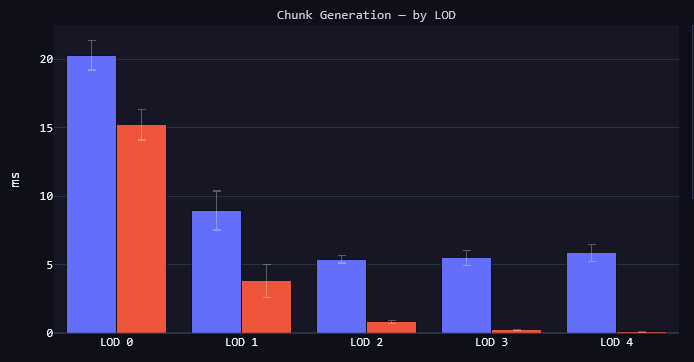
\includegraphics[width=1\textwidth]{Memoria/images/gpu_vs_cpu_chunk_256.png}
%    \caption{Comparison of GPU (left, blue) and CPU (right, orange) generation time of a chunk with resolution 256.}
%    \label{fig:gpu_vs_cpu_256}
%\end{figure}
%% ===================================================

%% ===================================================
\begin{figure}[H]
    \centering
    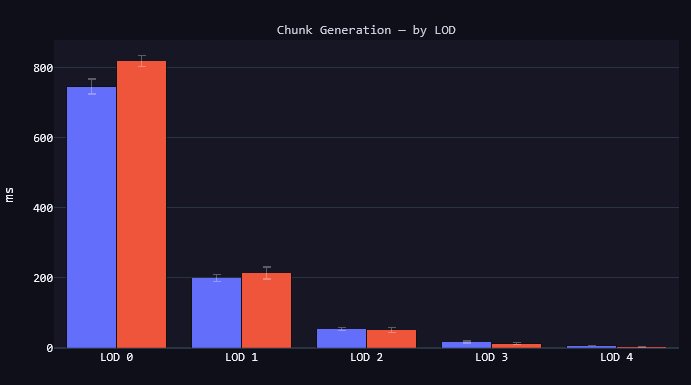
\includegraphics[width=1\textwidth]{Memoria/images/gpu_vs_cpu_chunk_2000.png}
    \caption{Comparison of GPU (left, blue) and CPU (right, orange) generation time of a chunk with resolution 2000.}
    \label{fig:gpu_vs_cpu_2000}
\end{figure}
%% ===================================================

\section{Architecture Comparison}
To complete the evaluation, a study of the system's behaviour on three distinct architectures has been performed.
%Para completar esta investigación, hemos decidido estudiar el comportamiento del sistema en tres arquitecturas razonablemente distintas.
They are:
\begin{itemize}
    \item Intel(R) Core(TM) i7-14700KF CPU and a NVIDIA GeForce RTX 4060 Ti GPU - Windows Desktop (the computer used in the other benchmarks).
    \item Apple M4 CPU and an Apple M4 (Apple9) (integrated) GPU - Apple MacBook Air 13.
    \item Intel(R) Core(TM) i7-13620H CPU and a NVIDIA GeForce RTX 4070 Laptop GPU - Windows Laptop.
\end{itemize}

The results confirm the previously observed behaviour, namely that GPU execution benefits heightmap generation and CPU benefits mesh generation (Compare Figures \ref{fig:all_gpu_heightmap}, \ref{fig:all_cpu_heightmap} and \ref{fig:all_gpu_chunk}, \ref{fig:all_cpu_chunk}).
Both Intel and NVIDIA combinations perform closely, with the Desktop GPU providing better performance in the large heightmap operations, while the Laptop seems to better perform in the mesh generation operations, where the communication overhead with the GPU dominates. 
The MacBook Air outperforms both of these greatly, which was expected in CPU performance, but surprises during GPU workloads. 
It even manages to outperform the CPU chunk generation path of the other architectures when running GPU.
This might hint towards the superiority of communications between CPU and GPU in the MacBook (as they are in the same chip), greatly outweighing the offloaded workload.
However, this is purely speculative and further profiling ought to be performed to validate the hypothesis. 

%% ===================================================
\begin{figure}[H]
    \centering
    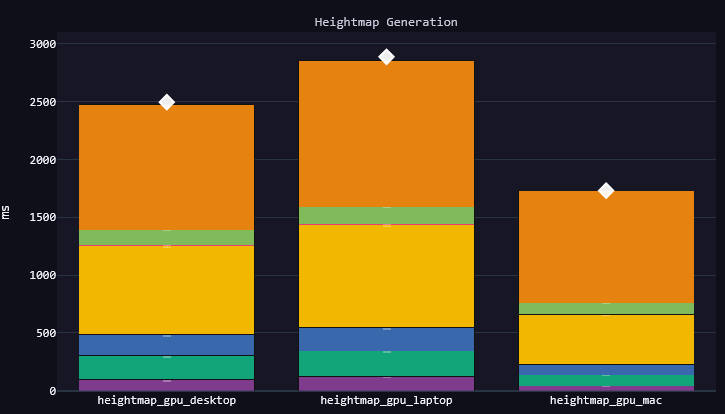
\includegraphics[width=.8\textwidth]{Memoria/images/all_gpu_heightmap2.png}
    \caption{Comparison of (from left to right) Desktop, Laptop and Mac GPU heightmap generation times. See Figure \ref{fig:heightmap_gen_cpu_gpu} for colour legend.}
    \label{fig:all_gpu_heightmap}
\end{figure}
%% ===================================================
%% ===================================================
\begin{figure}[H]
    \centering
    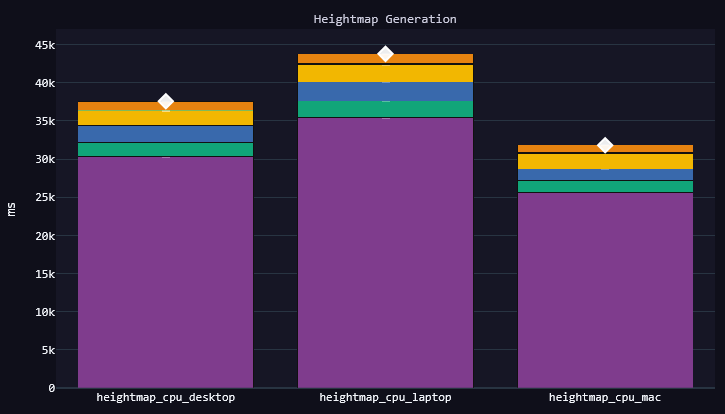
\includegraphics[width=.8\textwidth]{Memoria/images/all_cpu_heightmap2.png}
    \caption{Comparison of (from left to right) Desktop, Laptop and Mac CPU heightmap generation times. See Figure \ref{fig:heightmap_gen_cpu_gpu} for colour legend.}
    \label{fig:all_cpu_heightmap}
\end{figure}
%% ===================================================


%% ===================================================
\begin{figure}[H]
    \centering
    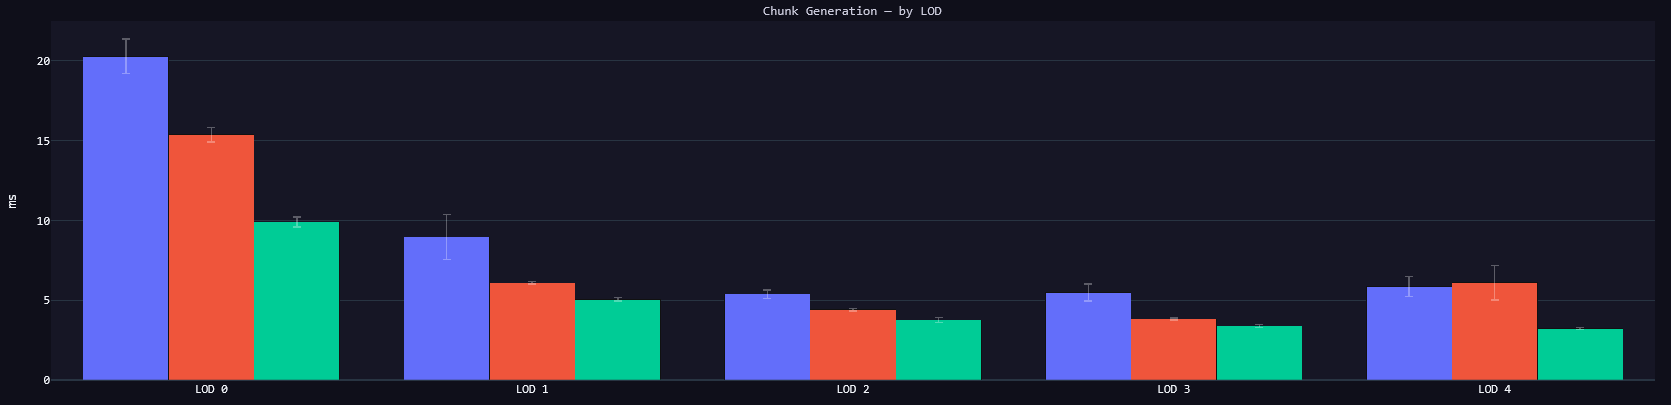
\includegraphics[width=1\textwidth]{Memoria/images/all_gpu_chunk_256.png}
    \caption{Comparison of (from left to right) Desktop, Laptop and Mac GPU chunk generation times on different LODs with base 256 resolution.}
    \label{fig:all_gpu_chunk}
\end{figure}
%% ===================================================
%% ===================================================
\begin{figure}[H]
    \centering
    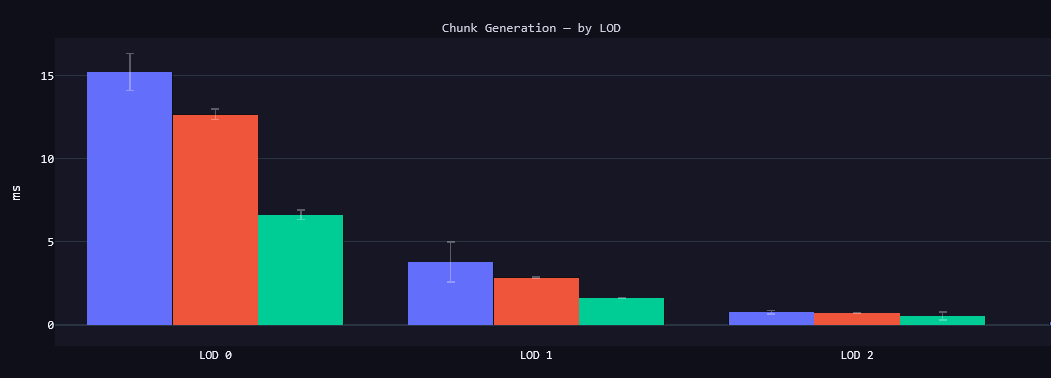
\includegraphics[width=1\textwidth]{Memoria/images/all_cpu_chunk_256.png}
    \caption{Comparison of (from left to right) Desktop, Laptop and Mac CPU chunk generation times on different LODs with base 256 resolution. Lower LODs are not included, as they cannot be properly distinguished in the image.}
    \label{fig:all_cpu_chunk}
\end{figure}
%% ===================================================



